%==============================================================================
% Sjabloon poster bachproef
%==============================================================================
% Gebaseerd op document class `a0poster' door Gerlinde Kettl en Matthias Weiser
% Aangepast voor gebruik aan HOGENT door Jens Buysse en Bert Van Vreckem
\documentclass[a0,portrait]{hogent-poster}
\usepackage{pgfplots} % used for graph generation 

% Info over de opleiding
\course{Bachelorproef}
\studyprogramme{toegepaste informatica}
\academicyear{2023-2024}
\institution{Hogeschool Gent, Valentin Vaerwyckweg 1, 9000 Gent}

% Info over de bachelorproef
\title{Het Web rekent op WebGPU}
\subtitle{Lokale inferentie met WebGPU ondersteunde browsers}
\author{Joris Van Duyse}
\email{joris.vanduyse@student.hogent.be}
\supervisor{Dhr. Thomas Desmedt}
\cosupervisor{Ing. Jonas Welvaert}

% Indien ingevuld, wordt deze informatie toegevoegd aan het einde van de
% abstract. Zet in commentaar als je dit niet wilt.
\specialisation{Enterprise- en Web-development}
\keywords{}
\projectrepo{https://github.com/JorisVanDuyseHogent/Bachelorproef-WebGPU-Ai}

\begin{document}

\maketitle

\begin{abstract}
  De opkomst van kunstmatige intelligentie \textit{(AI)} heeft de vraag naar \textit{server-side} rekenkracht verhoogd. Dit heeft een impact op kosten en het milieu. \textit{WebGPU} als nieuwe browser technologie kan een oplossing bieden voor deze uitdagingen door lokale rekenkracht beschikbaar te stellen. Dit onderzoek beschrijft en test de mogelijkheden van \textit{WebGPU} voor \textit{AI}-toepassingen. \textit{WebGPU} kan inferentie, essentieel voor \textit{AI}-modellen, lokaal uitvoeren, wat serverbelasting vermindert. Dit kan \textit{AI}-toepassingen sneller, gebruiksvriendelijker en goedkoper maken voor zowel gebruikers als bedrijven. Door \textit{WebGPU} te combineren met \textit{large language models}, wordt de prestatie vergeleken met bestaande technologieën, wat de potentie van \textit{WebGPU} voor \textit{AI}-ondersteuning op het web aantoont.
\end{abstract}

\begin{multicols}{2} % This is how many columns your poster will be broken into, a portrait poster is generally split into 2 columns

\section{Introductie}

De lancering van OpenAI's ChatGPT bracht een revolutionaire impact, waarvan de volledige schaal nog steeds moeilijk in te schatten is. AI-technologieën, zoals large language models, zullen de interactie van eindgebruikers met technologie sterk beïnvloeden. Browsertechnologie maakt AI toegankelijker zonder complex installatieproces, maar vereist dat AI-modellen operationeel blijven via grote datacentra.

Nieuwe technologieën zoals Progressive Web Apps (PWA's) vereenvoudigen de installatie van webapplicaties en kunnen kunstmatige intelligentie gebruiksvriendelijker maken. Echter, grootschalige implementatie van AI brengt hoge kosten voor cloudproviders met zich mee, die uiteindelijk de eindgebruikers betalen. Voor een duurzame en privacybewuste inzet van AI moet onderzocht worden hoe deze technologie efficiënt op grote schaal kan worden toegepast, waarbij de kosten en milieueffecten minimaal blijven.

\section{Experimenten}

De prestaties van WebGPU voor embedding modellen werden getest en vergeleken met Web Assembly (WASM) op verschillende hardwareconfiguraties binnen de browser. Daarnaast werd de uitvoeringstijd van het Whisper AI-model van OpenAI vergeleken tussen CPU, CUDA, en WebGPU implementaties op verschillende hardwareconfiguraties en modelgroottes. De testresultaten toonden aan dat WebGPU aanzienlijke prestatievoordelen biedt ten opzichte van CPU's, hoewel het niet even performant is als CUDA. Dit benadrukt de haalbaarheid en efficiëntie van WebGPU voor AI-inferentie in de browser, met voordelen zoals lokale verwerking en verhoogde privacy voor gebruikers.

Deze testen waren cruciaal om de capaciteiten en beperkingen van WebGPU te evalueren in vergelijking met traditionele technologieën. Ze geven inzicht in hoe WebGPU kan bijdragen aan de uitvoering en training van AI-modellen in een browseromgeving, met voordelen zoals lagere latentie en verbeterde privacy.

\section{Embedding test met WebAssembly en WebGPU}

De gemeten prestaties van verschillende hardwarecomponenten op basis van Floating Point Operations Per Second (FLOPS) worden in de volgende grafiek , met de Xeon E5-2680 v2 als referentiepunt. De resultaten tonen aan dat grafische kaarten aanzienlijk beter presteren dan CPU's voor deze embedding testen, vooral bij grotere batchgroottes. WebGPU presteert beter dan verwacht op basis van theoretische snelheden, vooral met de Nvidia GeForce GTX 1080 Ti, die de uitvoeringstijd tot 70 keer kan versnellen. Dit benadrukt de grote potentie van WebGPU voor het trainen van AI-modellen in de browser, terwijl CPU's beperkt concurreren met de parallelle rekenkracht van GPU's.

\pgfplotsset{width=15cm,compat=1.9}

% We will externalize the figures
% \tikzexternalize
\pgfplotsset{
  log ticks with fixed point,
}
\begin{tikzpicture}
    \begin{semilogxaxis}[
        title={Transformer benchmark fp32 WASM versus WebGPU},
        xlabel={Batch size},
        ylabel={Execution time in ms},
        xmin=1, xmax=64,
        ymin=0, ymax=70000,
        xtick={1,2,4,8,16,32, 64},
        ytick={1,10000,20000,30000,400000,50000,60000, 70000},
        legend pos=north west,
        ymajorgrids=true,
        grid style=dashed,
        scatter/classes={
            a={mark=square*,red},
            b={mark=triangle*,orange},
            c={mark=o,draw=blue},
            d={mark=square,green}
        },
        yticklabel style={
            /pgf/number format/fixed,
        },
        scaled y ticks=false
    ]
    
    \addplot[
        color=red,
        mark=square*
        ]
        coordinates {
            (1, 946.14)(2, 1923.12)(4, 3816.90)(8, 7653.00)(16, 15494.62)(32, 30901.40)(64, 61788.00)
        };
        \addlegendentry{WASM (fp32) Intel Xeon E5-2680 V2}
        
    \addplot[
        color=orange,
        mark=triangle*
        ]
        coordinates {
            (1, 747.10)(2, 1499.98)(4, 3014.38)(8, 5956.38)(16, 11807.70)(32, 24121.56)(64, 47769.14)
        };
        \addlegendentry{WASM (fp32) Intel Core i9-9980HK}
    \addplot[
        color=blue,
        mark=o
        ]
        coordinates {
            (1, 193.66)(2, 365.90)(4, 703.24)(8, 1393.12)(16, 2752.66)(32, 5510.74)(64, 10966.04)
        };
        \addlegendentry{WebGPU (fp32) Intel UHD Graphics 630}

    \addplot[
        color=green,
        mark=square
        ]
        coordinates {
            (1, 28.02)(2, 58.28)(4, 77.74)(8, 116.40)(16, 226.00)(32, 463.16)(64, 739.16)
        };
        \addlegendentry{WebGPU (fp32) Nvidia Geforce GTX 1080 Ti}
    \addplot [
        scatter,only marks,
        scatter src=explicit symbolic,
    ] table [x=x,y=y,meta=label] {plotdata/HuggingFaceWasmVSWebGPU.dat};

    \end{semilogxaxis}
\end{tikzpicture}

\section{Whisper-AI test met CUDA, CPU en WebGPU}

Het Whisper AI-model van OpenAI, met verschillende parametergroottes, biedt een basis voor prestatievergelijkingen, vooral vanwege geheugenbeperkingen. GPU's bieden hoge parallellisatie en geheugenbandbreedte, cruciaal voor inferentie. Testen met verschillende apparaten en modelgroottes (base, small, large) vergeleken de uitvoeringstijd van Whisper tussen CPU, CUDA en WebGPU. WebGPU toonde aanzienlijke voordelen ten opzichte van CPU's, hoewel niet even performant als CUDA.

Enkel bij een lage parameter grootte kunnen krachtige CPU's, zoals de Xeon E5-2680 v2 en v3, concurreren met de parallelle rekenkracht van GPU's. De WebGPU-implementatie presteert echter 53,4\%, 57,2\%, en 13,7\% langzamer dan CUDA voor respectievelijk de base, small, en large Whisper modellen. GPU's kunnen beter omgaan met grotere modellen door hun hogere VRAM-bandbreedte relatief tot processoren.

\pgfplotsset{width=12cm,compat=1.9}

\pgfplotsset{
  log ticks with fixed point,
}

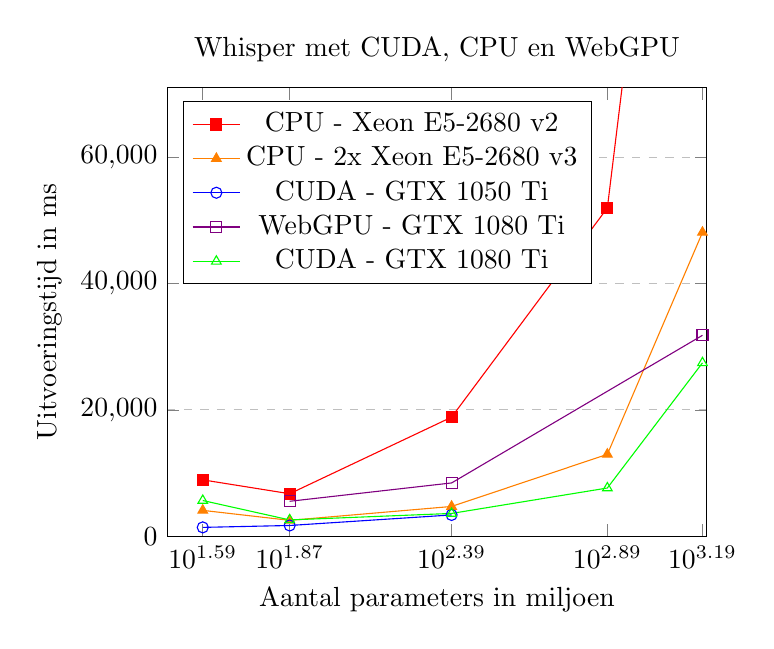
\begin{tikzpicture}
    \begin{semilogxaxis}[
        title={Whisper met CUDA, CPU en WebGPU},
        xlabel={Aantal parameters in miljoen},
        ylabel={Uitvoeringstijd in ms},
        xmin=30, xmax=1600,
        ymin=0, ymax=71000,
        xtick={39, 74, 244, 769, 1550},
        legend pos=north west,
        ymajorgrids=true,
        grid style=dashed,
        yticklabel style={
            /pgf/number format/fixed,
        },
        scaled y ticks=false
    ]
    \addplot[
            color=red,
            mark=square*
        ]
        coordinates {(39,8919)(74,6721)(244,18849)(769,51980)(1550,175378)};
        \addlegendentry{CPU - Xeon E5-2680 v2}
    \addplot[
        color=orange,
        mark=triangle*
        ]
        coordinates {(39,4088)(74,2508)(244,4706)(769,12963)(1550,48107)};
        \addlegendentry{CPU - 2x Xeon E5-2680 v3}
    \addplot[
            color=blue,
            mark=o
        ]
        coordinates {(39,1393)(74,1694)(244,3362)};
        \addlegendentry{CUDA - GTX 1050 Ti}
    \addplot[
            color=violet,
            mark=square
        ]
        coordinates {(74,5526)(244,8431)(1550,31814)};
        \addlegendentry{WebGPU - GTX 1080 Ti}
    \addplot[
            color=green,
            mark=triangle
        ]
        coordinates {(39,5647)(74,2574)(244,3602)(769,7629)(1550,27448)};
        \addlegendentry{CUDA - GTX 1080 Ti}
    \end{semilogxaxis}
\end{tikzpicture}

\section{Conclusies}

WebGPU biedt aanzienlijke voordelen voor AI-modellen in webapplicaties, met hoge prestaties en verbeterde privacy. Het ontgrendeld rekenkracht vergelijkbaar met traditionele low-level APIs, waardoor zowel inferentie als training van AI-modellen in de browser mogelijk is.

WebGPU vermindert de noodzaak voor externe diensten, verlaagt kosten, en beschermt gebruikersprivacy. De technology is reeds beschikbaar voor 70\% van internetgebruikers en kan hierdoor op grote schaal ingezet worden.

Hoewel nog in ontwikkeling, tonen nieuwe implementaties indrukwekkende resultaten, waardoor WebGPU aantrekkelijk is voor kleinschalige softwareoplossingen. Het maakt AI toegankelijker, met verbeterde privacy en minder afhankelijkheid van externe diensten. Hierdoor is WebGPU een aantrekkelijke keuze voor bedrijven en ontwikkelaars die willen profiteren van AI zonder de nadelen van complexe technologieën en privacyrisico's.

\section{Toekomstig onderzoek}

Toekomstig onderzoek over de privacy- en cybersecurityaspecten van WebGPU is nog vereist, waaronder de impact op digital fingerprinting en gevoeligheid voor side-channel attacks.

Daarnaast is het belangrijk om te onderzoeken hoe de technologische capaciteiten van eindgebruikersapparaten de prestaties van AI-modellen beïnvloeden. Browserfabrikanten en webontwikkelaars moeten verder werken aan het optimaliseren van WebGPU voor een breed scala aan apparaten om de volledige potentie van deze technologie te benutten.

\end{multicols}
\end{document}